% This file was created with tikzplotlib v0.9.12.
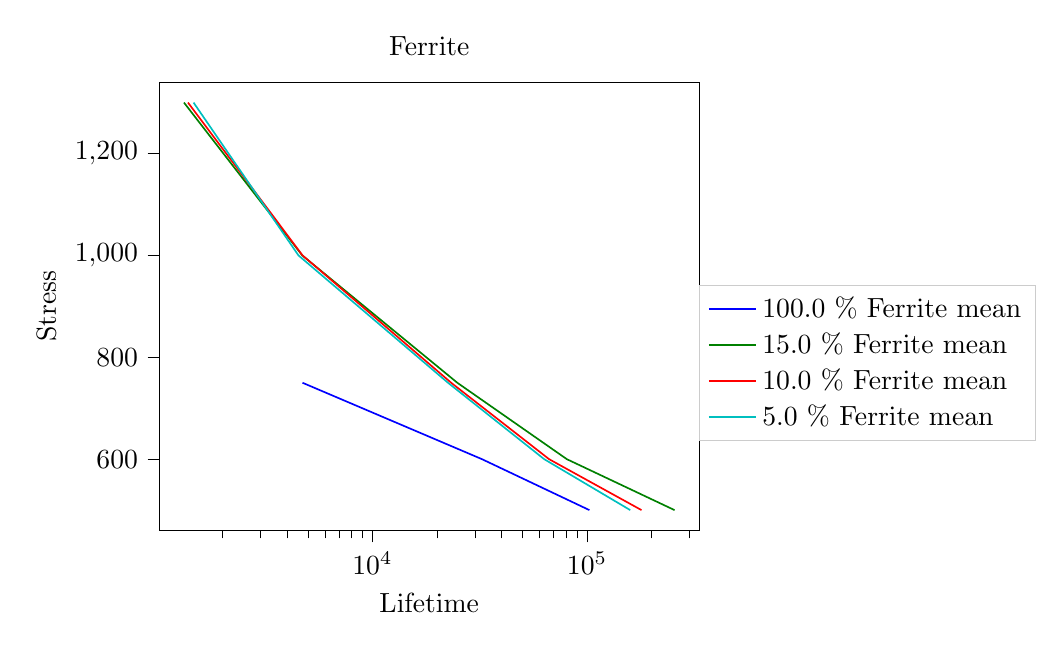
\begin{tikzpicture}

\definecolor{color0}{rgb}{0,0.75,0.75}

\begin{axis}[
legend cell align={left},
legend style={
  fill opacity=0.8,
  draw opacity=1,
  text opacity=1,
  at={(1,0.2)},
  anchor=south west,
  draw=white!80!black
},
log basis x={10},
tick align=outside,
tick pos=left,
title={Ferrite},
x grid style={white!69.0196078431373!black},
xlabel={Lifetime},
xmin=1017.48214066564, xmax=332982.351344122,
xmode=log,
xtick style={color=black},
y grid style={white!69.0196078431373!black},
ylabel={Stress},
ymin=460, ymax=1340,
ytick style={color=black}
]
\addplot [semithick, blue]
table {%
102622.170334593 500
32404.8001413774 600
4722.98589714715 750
nan 1000
nan 1300
};
\addlegendentry{100.0 \% Ferrite mean}
\addplot [semithick, green!50!black]
table {%
255922.1248858 500
80542.6590786477 600
24863.6607193755 750
4709.56292578244 1000
1323.8542615285 1300
};
\addlegendentry{15.0 \% Ferrite mean}
\addplot [semithick, red]
table {%
179512.287154513 500
66585.9521927846 600
23278.6976398127 750
4725.62535022617 1000
1382.34100811722 1300
};
\addlegendentry{10.0 \% Ferrite mean}
\addplot [semithick, color0]
table {%
159064.875765969 500
63175.443961492 600
22497.6654792561 750
4522.29082151709 1000
1467.25781559949 1300
};
\addlegendentry{5.0 \% Ferrite mean}
\end{axis}

\end{tikzpicture}
